\documentclass[aspectratio=169,10pt]{beamer}

% --- Typography & Encoding ---
\usepackage[T1]{fontenc}
\usepackage{lmodern}
\usepackage{booktabs}
\usepackage{tikz}
\usepackage{amsmath}
\usepackage{totcount}
\usetikzlibrary{arrows.meta, positioning, calc, shapes.misc, patterns, backgrounds}

% --- Theme Setup ---
\usetheme{default}
\useinnertheme{rectangles}
\setbeamertemplate{navigation symbols}{}
\setbeamertemplate{blocks}[rounded][shadow=false]

% --- Hadron Energy Brand Palette ---
\definecolor{HadronDark}{RGB}{33, 43, 54}      % Deep Slate/Navy
\definecolor{HadronBlue}{RGB}{0, 122, 204}     % Corporate Blue
\definecolor{HadronLight}{RGB}{245, 247, 250}  % Off-white background

% Status Colors
\definecolor{StatusRed}{RGB}{220, 53, 69}
\definecolor{StatusYellow}{RGB}{255, 193, 7}
\definecolor{StatusGreen}{RGB}{40, 167, 69}
\definecolor{StatusDark}{RGB}{52, 58, 64}
\definecolor{StatusOrange}{RGB}{253, 126, 20}

% --- Beamer Color Customization ---
\setbeamercolor{background canvas}{bg=white}
\setbeamercolor{frametitle}{bg=white, fg=HadronDark}
\setbeamercolor{title}{fg=white}
\setbeamercolor{subtitle}{fg=HadronBlue}
\setbeamercolor{structure}{fg=HadronBlue}

% Define Custom Block Color for Explanations
\setbeamercolor{explanation}{bg=HadronLight,fg=black}

% Font Sizes
\setbeamerfont{frametitle}{size=\large,series=\bfseries}
\setbeamerfont{block title}{size=\normalsize,series=\bfseries}

% Block styling
\setbeamercolor{block title}{bg=HadronDark, fg=white}
\setbeamercolor{block body}{bg=HadronLight, fg=black}

% --- Custom Graphics Definitions ---

\newcommand{\insertheaderlogo}{%
    \includegraphics[width=2.5cm, keepaspectratio]{media/hadron_logo.png}%
}

\newcommand{\statusbadge}[2]{%
    \tikz[baseline=(node.base)]{
        \node[fill=#1, text=white, rounded corners=3pt, inner sep=5pt, font=\bfseries\footnotesize, align=center, minimum width=2.5cm] (node) {#2};
    }%
}

% --- HEADER TEMPLATE ---
\setbeamertemplate{frametitle}{
    \nointerlineskip
    \begin{beamercolorbox}[wd=\paperwidth,ht=1.3cm,dp=0.6ex,leftskip=0.5cm,rightskip=0.5cm,sep=0cm,vmode]{frametitle}
        \centering
        \begin{minipage}[c][1.3cm][c]{\dimexpr\paperwidth-1cm\relax}
            \begin{minipage}[c]{0.72\textwidth}
                \raggedright
                \usebeamerfont{frametitle}\insertframetitle
            \end{minipage}%
            \hfill
            \begin{minipage}[c]{0.23\textwidth}
                \raggedleft
                \insertheaderlogo
            \end{minipage}
        \end{minipage}
    \end{beamercolorbox}
    \nointerlineskip
    {\color{HadronBlue}\hrule height 1pt}
}

% --- FOOTER TEMPLATE ---
\setbeamertemplate{footline}{
    \leavevmode%
    \hbox{%
    \begin{beamercolorbox}[wd=.333333\paperwidth,ht=2.25ex,dp=1ex,left]{author in head/foot}%
        \hspace*{2ex} \textcolor{gray}{\insertshortauthor}
    \end{beamercolorbox}%
    \begin{beamercolorbox}[wd=.333333\paperwidth,ht=2.25ex,dp=1ex,center]{title in head/foot}%
        \textcolor{gray}{\textbf{CORE SAFETY ANALYSIS}}
    \end{beamercolorbox}%
    \begin{beamercolorbox}[wd=.333333\paperwidth,ht=2.25ex,dp=1ex,right]{date in head/foot}%
        \textcolor{gray}{\insertframenumber{} / \the\numexpr\inserttotalframenumber-1\relax}\hspace*{2ex} 
    \end{beamercolorbox}}%
}

% --- Metadata ---
\title{Boiling Crisis \& Subchannel Analysis}
\subtitle{LWR Core Thermal Limits Assessment}
\author{Lander Ibarra}
\institute{Hadron Energy}
\date{\today}

\begin{document}

% ==========================================
% SLIDE 1: TITLE PAGE
% ==========================================
\begin{frame}[plain]
    \begin{tikzpicture}[remember picture,overlay]
        \fill[HadronDark] (current page.north west) rectangle (current page.south east);
        \node[anchor=north east] at (current page.north east) {
            \begin{tikzpicture}
                \fill[white] (0,0) rectangle (-4.0cm, -1.6cm); 
                \node[anchor=center] at (-2.0cm, -0.8cm) {
                    \includegraphics[width=3.0cm, keepaspectratio]{media/hadron_logo.png}
                };
            \end{tikzpicture}
        };
        \draw[HadronBlue, thick] ([yshift=-1.6cm]current page.north west) -- ([yshift=-1.6cm]current page.north east);
    \end{tikzpicture}
    
    \vspace{2.0cm} 
    \begin{center}
        \textcolor{HadronBlue}{\small \textbf{OPERATIONAL SAFETY BRIEFING}} \\[0.5em]
        {\Huge \textbf{\textcolor{white}{Boiling Crisis \&}}}\\
        {\Huge \textbf{\textcolor{white}{Subchannel Analysis}}}
        
        \vspace{0.5cm}
        \textcolor{white}{\large Engineering \& Safety}
        
        \vspace{1.5cm}
        \begin{columns}
            \column{0.5\textwidth}
            \raggedright
            \textcolor{gray}{\small PREPARED BY:}\\
            \textcolor{white}{\textbf{Lander Ibarra}}
            
            \column{0.5\textwidth}
            \raggedleft
            \textcolor{gray}{\small DATE:}\\
            \textcolor{white}{\textbf{\insertdate}}
        \end{columns}
    \end{center}
\end{frame}

\setcounter{framenumber}{0}

% ==========================================
% SLIDE 2: EXECUTIVE SUMMARY
% ==========================================
\begin{frame}[t]{Executive Summary}
    \vspace{0.5em}
    \begin{columns}[T,onlytextwidth]
        \column{0.65\textwidth}
        \begin{block}{Briefing Objectives}
            \begin{itemize}
                \item \textbf{Define the Threat:} Physics of boiling crisis (PWR DNB vs BWR Dryout).
                \item \textbf{Quantify Margins:} Deconstruct DNBR/CPR and statistical limits.
                \item \textbf{Methodology:} 3-Field discretization in modern subchannel codes.
            \end{itemize}
        \end{block}

        \begin{block}{Key Deliverables}
            \begin{itemize}
                \item Technical alignment for engineering \& operations.
                \item Validated transient response workflow.
            \end{itemize}
        \end{block}

        \column{0.32\textwidth}
        \centering
        \textbf{Operational State}
        \vspace{1em}
        \statusbadge{StatusGreen}{STATUS: GREEN \\ Normal Operation}
        \vspace{0.5em}
        \statusbadge{StatusYellow}{STATUS: YELLOW \\ Margin Erosion}
        \vspace{0.5em}
        \statusbadge{StatusRed}{STATUS: RED \\ Limit Exceeded}
    \end{columns}
\end{frame}

% ==========================================
% SLIDE 3: PHENOMENOLOGY
% ==========================================
\begin{frame}[t]{Phenomenology: The Boiling Transition}
    \begin{columns}[T,onlytextwidth]
        \column{0.58\textwidth}
        \textbf{The Definition:}
        A sudden transition from efficient nucleate boiling to an inefficient film boiling regime, causing a rapid, potentially destructive cladding temperature excursion.

        \vspace{1em}
        \textbf{Primary Drivers:}
        \begin{itemize}
            \item \textbf{Heat Flux $\uparrow$:} Power maneuvers, peaking factors, crud.
            \item \textbf{Cooling $\downarrow$:} Flow coastdown, depressurization, loss of subcooling.
            \item \textbf{Geometry:} Spacer grid deformation, flow blockage.
        \end{itemize}

        \column{0.38\textwidth}
        \begin{block}{Critical Terminology}
            Nucleate Boiling $\to$ Film Dryout $\to$ Wall Superheat.
            \vspace{0.5em}
            \emph{The transition is non-linear and cliff-like.}
        \end{block}

        \vspace{1em}
        \textbf{Safety Targets:}
        \begin{itemize} \small
            \item Cladding Integrity (PCT Limits).
            \item Fuel Rod Geometry (No ballooning).
            \item Regulatory Compliance (GDC).
        \end{itemize}
    \end{columns}
\end{frame}

% ==========================================
% SLIDE 4: CHF VS BOILING CRISIS
% ==========================================
\begin{frame}[t]{CHF vs. Boiling Crisis}
    \begin{columns}[T,onlytextwidth]
        \column{0.50\textwidth}
        \begin{block}{Terminology}
            \begin{itemize}
                \item \textbf{CHF (Critical Heat Flux):} The maximum heat flux where the wall maintains continuous liquid contact.
                \item \textbf{Boiling Crisis:} The post-CHF regime characterized by vapor blanketing.
            \end{itemize}
        \end{block}

        \vspace{1em}
        \textbf{Regime Classification:}
        \begin{description}
            \item[PWR:] \textbf{DNB} (Departure from Nucleate Boiling). Subcooled/Low quality.
            \item[BWR:] \textbf{Dryout}. High quality annular flow (liquid film depletion).
        \end{description}

        \column{0.48\textwidth}
        \begin{center}
            \includegraphics[width=\linewidth,height=0.7\textheight,keepaspectratio]{media/A_comparative_diagram_in_the_field_of_nuclear_reac.png}
            \vspace{0.5em}
            {\tiny \color{gray} Comparison of bubble dynamics (Source: nuclear-power.com)}
        \end{center}
    \end{columns}
\end{frame}

% ==========================================
% SLIDE 5: REGIME MAP
% ==========================================
\begin{frame}[t]{Regime Map: Operational Parameters}
    \begin{columns}[T,onlytextwidth]
        \column{0.6\textwidth}
        \begin{block}{Governing Physics}
            \begin{enumerate}
                \item \textbf{Pressure:} Influences saturation temp, fluid properties, and bubble dynamics.
                \item \textbf{Mass Flux ($G$):} Drives convective cooling, entrainment, and rewetting.
                \item \textbf{Quality ($x$) / Subcooling:} Defines the thermodynamic state along the boiling curve.
            \end{enumerate}
        \end{block}

        \vspace{1em}
        \textbf{Heuristics:}
        \begin{itemize}
            \item \textbf{PWR DNB:} Driven by local heat flux vs. bubble crowding.
            \item \textbf{BWR Dryout:} Driven by integral power vs. film inventory.
        \end{itemize}

        \column{0.35\textwidth}
        \textbf{Control Room Monitors}
        \begin{itemize} \small
            \item Pressurizer Pressure
            \item Loop/Core Flow
            \item Axial Flux Difference (AFD)
            \item $F_{\Delta H}$ / $F_Q$
        \end{itemize}
        
        \vspace{1cm}
        \statusbadge{StatusYellow}{RULE: Margin $\downarrow$ if Power $\uparrow$ or Flow $\downarrow$}
    \end{columns}
\end{frame}

% ==========================================
% SLIDE 6: PWR DEEP DIVE
% ==========================================
\begin{frame}[t]{PWR Deep Dive: DNB (Low-Quality)}
    \begin{columns}[T,onlytextwidth]
        \column{0.45\textwidth}
        \textbf{Mechanism:}
        \begin{itemize}
            \item Intense nucleate boiling creates bubble crowding at the wall.
            \item Liquid supply to the surface is choked off.
            \item Vapor blanket insulates the rod, causing temperature excursion.
        \end{itemize}

        \vspace{1em}
        \textbf{Location:}
        \begin{itemize}
            \item Hot channel (highest radial peaking).
            \item Usually slightly downstream of peak power (enthalpy effect).
        \end{itemize}

        \column{0.53\textwidth}
        \centering
        \includegraphics[height=0.75\textheight,width=\linewidth,keepaspectratio,trim=0 0 360 0,clip]{media/Dryout-DNB-min.png}
    \end{columns}
\end{frame}

% ==========================================
% SLIDE 7: BWR DEEP DIVE
% ==========================================
\begin{frame}[t]{BWR Deep Dive: Dryout (High-Quality)}
    \begin{columns}[T,onlytextwidth]
        \column{0.45\textwidth}
        \textbf{Mechanism:}
        \begin{itemize}
            \item Annular flow regime: Vapor core, liquid film on wall.
            \item Film is depleted by evaporation and entrainment (droplet stripping).
            \item When film thickness $\to$ 0, dryout occurs.
        \end{itemize}

        \vspace{1em}
        \textbf{Location:}
        \begin{itemize}
            \item Typically near the top of the bundle (highest quality).
            \item Strongly dependent on spacer grid "rewetting" effects.
        \end{itemize}

        \column{0.53\textwidth}
        \centering
        \includegraphics[height=0.75\textheight,width=\linewidth,keepaspectratio,trim=360 0 0 0,clip]{media/Dryout-DNB-min.png}
    \end{columns}
\end{frame}

% ==========================================
% SLIDE 8: THE CLIFF
% ==========================================
\begin{frame}[t]{The Heat Transfer Cliff}
    \begin{columns}[T,onlytextwidth]
        \column{0.50\textwidth}
        \textbf{Why CHF Matters:}
        \begin{itemize}
            \item \textbf{Pre-CHF:} Nucleate boiling provides high Heat Transfer Coefficient (HTC).
            \item \textbf{At CHF:} Critical limit is reached.
            \item \textbf{Post-CHF:} Film boiling (vapor insulation) drops HTC by orders of magnitude.
        \end{itemize}
        
        \vspace{1.5cm}
        \statusbadge{StatusRed}{CRITICAL \\ Small hydraulic change = Large $\Delta T$}

        \column{0.45\textwidth}
        \centering
        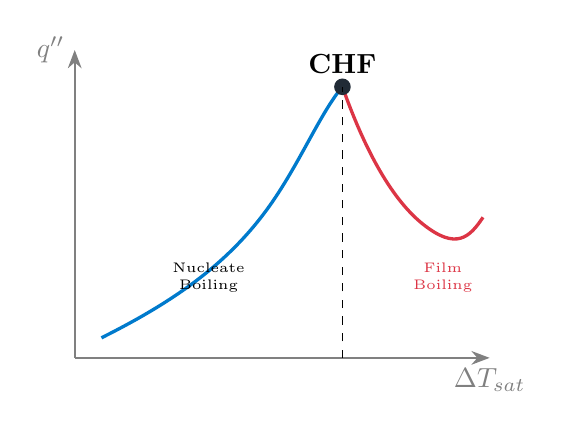
\begin{tikzpicture}[x=0.85cm,y=0.85cm]
          \draw[-{Stealth}, thick, color=gray] (0,0) -- (6.2,0) node[below] {$\Delta T_{sat}$};
          \draw[-{Stealth}, thick, color=gray] (0,0) -- (0,4.6) node[left] {$q''$};
          \draw[very thick, HadronBlue] (0.4,0.3) .. controls (1.6,0.9) and (2.4,1.5) .. (3.0,2.4)
                       .. controls (3.4,3.0) and (3.7,3.7) .. (4.0,4.05);
          \draw[very thick, StatusRed] (4.0,4.05) .. controls (4.3,3.2) and (4.7,2.4) .. (5.2,2.0)
                       .. controls (5.7,1.6) and (5.9,1.8) .. (6.1,2.1);
          \fill[HadronDark] (4.0,4.05) circle (3pt);
          \draw[dashed] (4.0,0) -- (4.0,4.05);
          \node[above] at (4.0,4.1) {\textbf{CHF}};
          \node[align=center, font=\tiny] at (2.0,1.2) {Nucleate\\Boiling};
          \node[align=center, font=\tiny, color=StatusRed] at (5.5,1.2) {Film\\Boiling};
        \end{tikzpicture}
    \end{columns}
\end{frame}

% ==========================================
% SLIDE 9: SAFETY LIMITS
% ==========================================
\begin{frame}[t]{Safety Limits: DNBR vs. CPR}
    \begin{columns}[T,onlytextwidth]
        \column{0.48\textwidth}
        \begin{block}{PWR: DNBR (Ratio)}
            \[ \text{DNBR} = \frac{\text{Predicted CHF}}{\text{Actual Heat Flux}} \]
            \begin{itemize}
                \item \textbf{Goal:} Maintain $> \text{Limit}$ (e.g., 1.30).
                \item \emph{Physical Meaning:} Margin against rewet failure.
            \end{itemize}
        \end{block}

        \column{0.48\textwidth}
        \begin{block}{BWR: CPR (Ratio)}
            \[ \text{CPR} = \frac{\text{Critical Power}}{\text{Bundle Power}} \]
            \begin{itemize}
                \item \textbf{Goal:} Maintain $> \text{OLMCPR}$.
                \item \emph{Physical Meaning:} Margin against film dryout.
            \end{itemize}
        \end{block}
    \end{columns}
    
    \vspace{1em}
    \centering
    \statusbadge{StatusYellow}{Action: Investigate any downward trend.}
\end{frame}

% ==========================================
% SLIDE 10: SCALING CONSIDERATIONS
% ==========================================
\begin{frame}[t]{Scaling Considerations: From Core to Pin}
    \begin{columns}[T,onlytextwidth]
        \column{0.55\textwidth}
        \textbf{The Resolution Requirement:}
        Core and assembly-level thermal-hydraulics "smear" properties, masking the local extremes where DNB actually occurs. To accurately model safety limits, the resolution must be refined.
        
        \vspace{1em}
        \textbf{Nodalization Hierarchy:}
        \begin{enumerate}
            \item \textbf{Core Level:} Coarse nodes (1 node/assembly). Sets global Pressure \& Flow boundary conditions.
            \item \textbf{Assembly Level:} Identifies the "Hot Assembly" but misses intra-assembly flow redistribution.
            \item \textbf{Subchannel Level:} The required scale to capture \textbf{complex local effects}:
            \begin{itemize} \scriptsize
                \item Local mixing from mixing vanes.
                \item Radial crossflows within and between assemblies.
            \end{itemize}
        \end{enumerate}

        \column{0.40\textwidth}
        \centering
        \includegraphics[width=\linewidth, keepaspectratio]{media/nodalization.jpg}
        \vspace{0.2em}
        {\tiny \color{HadronDark} Integrated Scaling Hierarchy}
    \end{columns}
\end{frame}

% ==========================================
% SLIDE 11: SUBCHANNEL ANALYSIS METHOD
% ==========================================
\begin{frame}[t]{Subchannel Analysis: The Method}
    \begin{columns}[T,onlytextwidth]
        \column{0.6\textwidth}
        \textbf{Overview:}
        A thermal-hydraulic modeling approach that discretizes fuel assemblies into parallel, coupled flow channels ("subchannels") to solve conservation equations.

        \vspace{1em}
        \textbf{Advantages over CFD:}
        \begin{itemize}
            \item Computational efficiency allows full-core analysis.
            \item Validated correlations for mixing and CHF.
            \item Industry standard (VIPRE, COBRA, CTF).
        \end{itemize}

        \column{0.35\textwidth}
        \begin{block}{Key Outputs}
            \begin{itemize}
                \item Minimum DNBR/MCPR
                \item Local Quality/Void
                \item Mass Velocity ($G_{local}$)
            \end{itemize}
        \end{block}
        \vspace{1em}
        \statusbadge{StatusYellow}{"Bundle Weather Forecast"}
    \end{columns}
\end{frame}

% ==========================================
% SLIDE 12: DISCRETIZATION
% ==========================================
\begin{frame}[t]{Discretization: Subchannel vs. System Level}
    \vspace{-0.5em}
    \begin{columns}[T,onlytextwidth]
        \column{0.45\textwidth}
        \begin{center}
            \textbf{System Level (RELAP/TRACE)}
            \vspace{0.5em}
            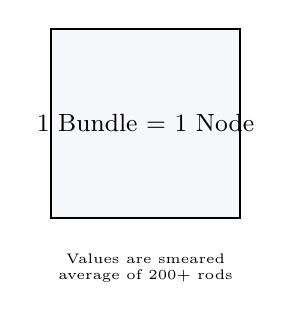
\begin{tikzpicture}[scale=0.8]
                \draw[thick, fill=HadronLight] (0,0) rectangle (3,3);
                \node at (1.5, 1.5) {\small 1 Bundle = 1 Node};
                \node[font=\tiny, align=center] at (1.5, -0.8) {Values are smeared\\average of 200+ rods};
            \end{tikzpicture}
        \end{center}
        \vspace{0.5em}
        \small
        \begin{itemize}
            \item \textbf{Resolution:} Coarse (1-D flow).
            \item \textbf{Use Case:} LOCA, plant transients.
            \item \textbf{Blind Spot:} No local peaking visibility.
        \end{itemize}

        \column{0.45\textwidth}
        \begin{center}
            \textbf{Subchannel (VIPRE/CTF)}
            \vspace{0.5em}
            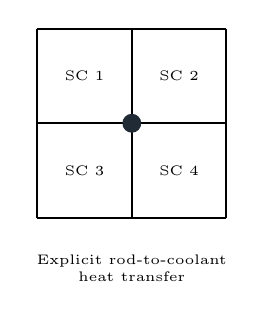
\begin{tikzpicture}[scale=0.8]
                \draw[thick, step=1.5] (0,0) grid (3,3);
                \node at (0.75, 2.25) {\tiny SC 1}; \node at (2.25, 2.25) {\tiny SC 2};
                \node at (0.75, 0.75) {\tiny SC 3}; \node at (2.25, 0.75) {\tiny SC 4};
                \fill[HadronDark] (1.5,1.5) circle (0.15); 
                \node[font=\tiny, align=center] at (1.5, -0.8) {Explicit rod-to-coolant\\heat transfer};
            \end{tikzpicture}
        \end{center}
        \vspace{0.5em}
        \small
        \begin{itemize}
            \item \textbf{Resolution:} Fine (pin-level).
            \item \textbf{Use Case:} DNB/Dryout margin.
            \item \textbf{Key Physics:} Turbulent mixing.
        \end{itemize}
    \end{columns}
\end{frame}

% ==========================================
% SLIDE 13: BUNDLE NODALIZATION
% ==========================================
\begin{frame}[t]{Bundle Nodalization: Subchannels \& Gaps}
    \begin{columns}[T,onlytextwidth]
        \column{0.50\textwidth}
        \textbf{Definitions:}
        \begin{itemize}
            \item \textbf{Subchannel ($i$):} The flow area between rods (Control Volume). 
            \item \textbf{Gap ($k$):} Lateral connection between subchannels where crossflow ($w_{ij}$) occurs.
            \item \textbf{Rod:} Heat source ($q''$).
        \end{itemize}
        \vspace{0.5em}
        {\small \textit{Subchannel codes discretize the entire core into thousands of these parallel channels to find local limits.}}

        \column{0.45\textwidth}
        \centering
        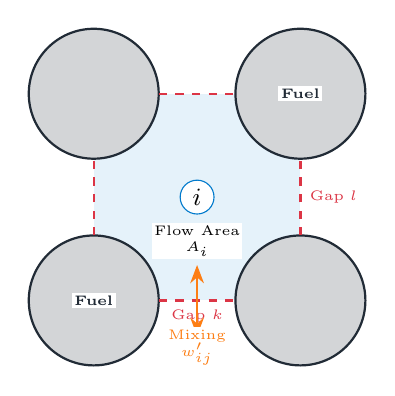
\begin{tikzpicture}[scale=0.75]
            \def\P{3.5}
            \def\R{1.1}
            \fill[HadronBlue!10] (0,0) rectangle (\P,\P);
            \foreach \pos in {(0,0), (\P,0), (0,\P), (\P,\P)} {
                \filldraw[fill=HadronDark!20, draw=HadronDark, thick] \pos circle (\R);
            }
            \node[font=\bfseries\tiny, color=HadronDark, fill=white, inner sep=1pt] at (0,0) {Fuel};
            \node[font=\bfseries\tiny, color=HadronDark, fill=white, inner sep=1pt] at (\P,\P) {Fuel};
            \draw[dashed, StatusRed, thick] (\R, 0) -- (\P-\R, 0) node[midway, below=2pt, font=\tiny, fill=white, inner sep=1pt] {Gap $k$};
            \draw[dashed, StatusRed, thick] (\R, \P) -- (\P-\R, \P);
            \draw[dashed, StatusRed, thick] (0, \R) -- (0, \P-\R);
            \draw[dashed, StatusRed, thick] (\P, \R) -- (\P, \P-\R) node[midway, right=2pt, font=\tiny, fill=white, inner sep=1pt] {Gap $l$};
            \draw[{Stealth}-{Stealth}, thick, StatusOrange] (\P/2, -0.6) -- (\P/2, 0.6);
            \node[font=\tiny, color=StatusOrange, align=center, fill=white, inner sep=1pt] at (\P/2, -0.8) {Mixing\\$w'_{ij}$};
            \node[circle, fill=white, draw=HadronBlue, inner sep=2pt] (c) at (\P/2, \P/2) {\small $i$};
            \node[align=center, font=\tiny, below=0.1cm of c, fill=white, inner sep=1pt] {Flow Area\\$A_i$};
        \end{tikzpicture}
    \end{columns}
\end{frame}

% ==========================================
% SLIDE 14: GOVERNING EQUATIONS (MIXTURE)
% ==========================================
\begin{frame}[t]{Subchannel Governing Equations (Mixture Model)}
    \begin{columns}[T,onlytextwidth]
        \column{0.62\textwidth}
        \textbf{Conservation Laws (Control Volume $i$):}
        \vspace{-0.3em}
        \begin{block}{Mass Conservation}
            \small
            \[ \frac{\partial \rho_i}{\partial t} + \frac{\partial (\rho_i u_i)}{\partial z} + \sum_j w_{ij} = 0 \]
        \end{block}
        \vspace{-0.3em}
        \begin{block}{Momentum Conservation (Axial)}
            \small
            \[ \frac{\partial P}{\partial z} = - \frac{\partial (\rho u^2)}{\partial z} - \left[ \frac{f}{D_h} + K \right] \frac{\rho u^2}{2} - \rho g - \sum_j w_{ij} u^* \]
        \end{block}
        \vspace{-0.3em}
        \begin{block}{Energy Conservation}
            \small
            \[ \frac{\partial (\rho_i h_i)}{\partial t} + \frac{\partial (\rho_i u_i h_i)}{\partial z} = q'_{rod} - \sum_j (w_{ij} h^* + w'_{ij}\Delta h) \]
        \end{block}

        \column{0.35\textwidth}
        \vspace{1em}
        \textbf{Key Terms}
        \scriptsize
        \begin{itemize}
            \item $w_{ij}$: Diversion crossflow (driven by $\Delta P$).
            \item $w'_{ij}$: Turbulent mixing (driven by $\Delta h$).
            \item $f, K$: Friction \& Form loss.
        \end{itemize}
    \end{columns}
\end{frame}

% ==========================================
% SLIDE 15: MIXING & CROSSFLOW
% ==========================================
\begin{frame}[t]{Mixing \& Crossflow: The Secret Sauce}
    \begin{columns}[T,onlytextwidth]
        \column{0.55\textwidth}
        \begin{block}{Turbulent Mixing ($w'$)}
            Net zero mass exchange ($\dot{m}_{net} = 0$). Swaps energy and momentum. 
            \emph{Effect:} Cools the hot pin by sharing heat with cooler neighbors.
        \end{block}
        
        \begin{block}{Diversion Crossflow ($w$)}
            Net mass movement ($\dot{m}_{net} \neq 0$) driven by pressure gradients (e.g., blockage, boiling expansion).
        \end{block}
        
        \vspace{0.5em}
        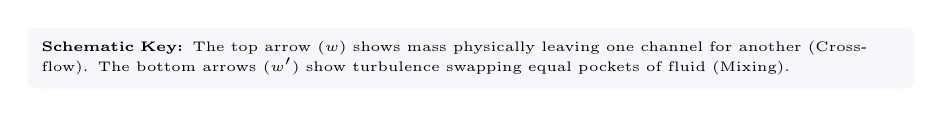
\begin{tikzpicture}
            \node[fill=HadronLight, rounded corners=3pt, inner sep=5pt, text width=0.9\linewidth, font=\tiny] {
                \textbf{Schematic Key:} The top arrow ($w$) shows mass physically leaving one channel for another (Crossflow). The bottom arrows ($w'$) show turbulence swapping equal pockets of fluid (Mixing).
            };
        \end{tikzpicture}

        \column{0.42\textwidth}
        \centering
        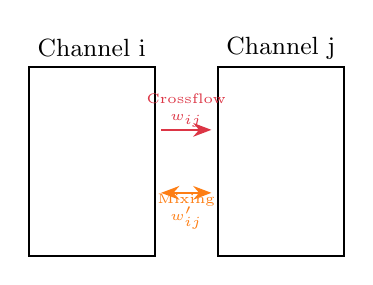
\begin{tikzpicture}[scale=0.8]
            \draw[thick] (0,0) rectangle (2,3);
            \node at (1,3.3) {\small Channel i};
            \draw[thick] (3,0) rectangle (5,3);
            \node at (4,3.3) {\small Channel j};
            \draw[-{Stealth}, thick, StatusRed] (2.1, 2.0) -- (2.9, 2.0);
            \node[font=\tiny, StatusRed, align=center] at (2.5, 2.3) {Crossflow\\$w_{ij}$};
            \draw[{Stealth}-{Stealth}, thick, StatusOrange] (2.1, 1.0) -- (2.9, 1.0);
            \node[font=\tiny, StatusOrange, align=center] at (2.5, 0.7) {Mixing\\$w'_{ij}$};
        \end{tikzpicture}
    \end{columns}
\end{frame}

% ==========================================
% SLIDE 16: ADVANCED MODELING (3-FIELD)
% ==========================================
\begin{frame}[t]{Advanced Modeling: The 3-Field Approach}
    \begin{columns}[T,onlytextwidth]
        \column{0.58\textwidth}
        \textbf{Beyond Homogeneous Equilibrium:}
        Standard models assume liquid and vapor move together. For BWR dryout, we need more physics.
        
        \vspace{1em}
        \textbf{The 3 Fields:}
        \begin{enumerate}
            \item \textbf{Continuous Liquid:} The film on the wall.
            \item \textbf{Entrained Liquid:} Droplets in the core.
            \item \textbf{Vapor:} The gaseous core.
        \end{enumerate}

        \column{0.38\textwidth}
        \centering
        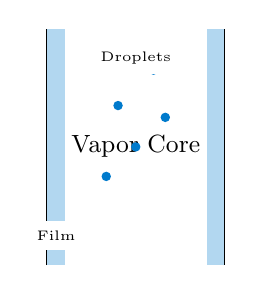
\begin{tikzpicture}[scale=0.75]
            \draw[thick] (0,0) -- (0,4);
            \draw[thick] (3,0) -- (3,4);
            \fill[HadronBlue!30] (0,0) rectangle (0.3,4);
            \fill[HadronBlue!30] (2.7,0) rectangle (3,4);
            \node at (1.5, 2) {\small Vapor Core};
            \foreach \x in {1,1.5,2} \fill[HadronBlue] (\x, \x+0.5) circle (0.08);
            \foreach \x in {1.2,1.8} \fill[HadronBlue] (\x, \x+1.5) circle (0.08);
            \node[font=\tiny, align=center, fill=white] at (0.15, 0.5) {Film};
            \node[font=\tiny, align=center, fill=white] at (1.5, 3.5) {Droplets};
        \end{tikzpicture}
    \end{columns}
\end{frame}

% ==========================================
% SLIDE 17: 3-FIELD MASS CONSERVATION
% ==========================================
\begin{frame}[t]{3-Field Equations: Mass Conservation}
    \small % Reduced text size
    \textbf{Three separate mass balances per node:}
    
    \begin{block}{1. Vapor Mass}
        \[ \frac{\partial (\alpha_v \rho_v)}{\partial t} + \nabla \cdot (\alpha_v \rho_v \vec{v}_v) = \Gamma_{vap} \]
        {\tiny Vapor generation from evaporation.}
    \end{block}
    
    \begin{block}{2. Liquid Film Mass}
        \[ \frac{\partial (\alpha_f \rho_f)}{\partial t} + \nabla \cdot (\alpha_f \rho_f \vec{v}_f) = \textcolor{StatusGreen}{D} - \textcolor{StatusRed}{E} - \Gamma_{film} \]
        {\tiny $\mathbf{D}$: Deposition of drops to film. $\mathbf{E}$: Entrainment of film to drops.}
    \end{block}
    
    \begin{block}{3. Entrained Droplet Mass}
        \[ \frac{\partial (\alpha_d \rho_d)}{\partial t} + \nabla \cdot (\alpha_d \rho_d \vec{v}_d) = \textcolor{StatusRed}{E} - \textcolor{StatusGreen}{D} - \Gamma_{drops} \]
    \end{block}
    
    \vspace{0.2em}
    \centering
    \statusbadge{StatusYellow}{Dryout happens when Film Mass $\to$ 0.}
\end{frame}

% ==========================================
% SLIDE 18: 3-FIELD MOMENTUM BALANCE
% ==========================================
\begin{frame}[t]{3-Field Equations: Momentum Balance}
    \begin{columns}[T,onlytextwidth]
        \column{0.6\textwidth}
        \textbf{Momentum Complexity:}
        We solve momentum for each field, allowing different velocities ($v_v \neq v_d \neq v_f$).
        
        \vspace{1em}
        \begin{block}{Interfacial Drag}
            The fields interact through drag forces:
            \[ F_{i} = C_D \frac{1}{2} \rho (v_{rel}) |v_{rel}| A_{int} \]
            \begin{itemize}
                \item Vapor drags droplets up.
                \item Vapor shears the film surface.
            \end{itemize}
        \end{block}

        \column{0.35\textwidth}
        \textbf{Operational Impact}
        \vspace{0.5em}
        
        If vapor velocity is very high, it shears the film surface, increasing \textbf{Entrainment (E)}.
        \vspace{1em}
        
        High Entrainment $\to$ Thinner Film $\to$ Earlier Dryout.
    \end{columns}
\end{frame}

% ==========================================
% SLIDE 19: 3-FIELD ENERGY BALANCE
% ==========================================
\begin{frame}[t]{3-Field Equations: Energy Balance}
    \textbf{Where does the heat go?}
    
    \begin{block}{Film Energy Equation}
        Heat from the rod enters the liquid film.
        \begin{itemize}
            \item If $T_{film} < T_{sat}$: Sensible heating.
            \item If $T_{film} = T_{sat}$: Evaporation ($\Gamma_{film}$).
        \end{itemize}
    \end{block}
    
    \begin{block}{Vapor/Droplet Energy}
        Typically, droplets are assumed to be at $T_{sat}$. 
        Vapor can become \textbf{superheated} even if droplets exist (non-equilibrium), but in standard dryout analysis, we focus on the film depletion limit.
    \end{block}
    
    \vspace{1em}
    \centering
    \statusbadge{StatusDark}{Critical Logic: Dryout = Integrated Film Depletion}
\end{frame}

% ==========================================
% SLIDE 20: CLOSURE MODELS
% ==========================================
\begin{frame}[t]{Closure Models: The Entrainment/Deposition War}
    The accuracy of a 3-field code (like COBRA-TF) depends entirely on these empirical models:
    
    \vspace{1em}
    \begin{columns}[T,onlytextwidth]
        \column{0.48\textwidth}
        \begin{block}{Entrainment (E)}
            \begin{itemize}
                \item \textbf{Driver:} Vapor shear vs. Surface tension.
                \item \textbf{Effect:} Rips liquid off the wall.
                \item \textbf{Bad for margins.}
            \end{itemize}
        \end{block}

        \column{0.48\textwidth}
        \begin{block}{Deposition (D)}
            \begin{itemize}
                \item \textbf{Driver:} Turbulent diffusion of drops.
                \item \textbf{Effect:} Returns liquid to the wall.
                \item \textbf{Good for margins.}
            \end{itemize}
        \end{block}
    \end{columns}
    
    \vspace{1em}
    \textbf{Spacer Grids:} Modern spacers are designed to maximize \textbf{D} (Deposition) to replenish the film.
\end{frame}

% ==========================================
% SLIDE 21: UNCERTAINTY CHALLENGE
% ==========================================
\begin{frame}[t]{The Uncertainty Challenge}
    \begin{columns}[T,onlytextwidth]
        \column{0.50\textwidth}
        \textbf{The Problem:}
        Calculating CHF with "nominal" values assumes a perfect world. 
        
        \vspace{1em}
        \textbf{Sources of Uncertainty:}
        \begin{itemize}
            \item \textbf{Plant Data:} Power, Flow, Temp ($\pm 2\%$).
            \item \textbf{Manufacturing:} Rod pitch, Diameter.
            \item \textbf{Code/Model:} Correlation scatter.
        \end{itemize}
        
        \vspace{1em}
        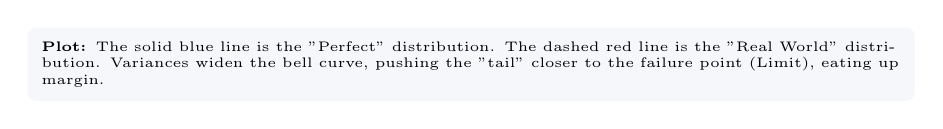
\begin{tikzpicture}
            \node[fill=HadronLight, rounded corners=3pt, inner sep=5pt, text width=0.9\linewidth, font=\tiny] {
                \textbf{Plot:} The solid blue line is the "Perfect" distribution. The dashed red line is the "Real World" distribution. Variances widen the bell curve, pushing the "tail" closer to the failure point (Limit), eating up margin.
            };
        \end{tikzpicture}

        \column{0.48\textwidth}
        \centering
        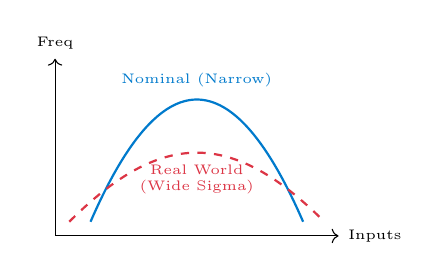
\begin{tikzpicture}[scale=0.9]
            \draw[->] (0,0) -- (4,0) node[right] {\tiny Inputs};
            \draw[->] (0,0) -- (0,2.5) node[above] {\tiny Freq};
            \draw[thick, HadronBlue] (0.5,0.2) .. controls (1.5,2.5) and (2.5,2.5) .. (3.5,0.2);
            \node[HadronBlue, font=\tiny] at (2, 2.2) {Nominal (Narrow)};
            \draw[thick, StatusRed, dashed] (0.2,0.2) .. controls (1.5,1.5) and (2.5,1.5) .. (3.8,0.2);
            \node[StatusRed, font=\tiny, align=center] at (2, 0.8) {Real World\\(Wide Sigma)};
        \end{tikzpicture}
        \vspace{0.5em}
        \statusbadge{StatusRed}{Impact: Margin $\downarrow$ significantly}
    \end{columns}
\end{frame}

% ==========================================
% SLIDE 22: STATISTICAL METHODOLOGY
% ==========================================
\begin{frame}[t]{Statistical Methodology: RTDP vs. Monte Carlo}
    \begin{columns}[T,onlytextwidth]
        \column{0.50\textwidth}
        \begin{block}{RTDP (Revised Thermal Design Procedure)}
            \begin{itemize}
                \item Used in PWRs.
                \item Combines uncertainties using Root Sum Square (RSS) statistics.
                \item Result: A single "Design Limit DNBR" (e.g., 1.25).
            \end{itemize}
        \end{block}
        
        \begin{block}{Monte Carlo Sampling}
            \begin{itemize}
                \item Run subchannel code a number of times based on the desired confidence interval.
                \item Randomly sample inputs from PDFs.
                \item Determine true failure probability.
            \end{itemize}
        \end{block}

        \column{0.48\textwidth}
        \centering
        % Top: Process Flow (TikZ) - Scaled down to fit
        \scalebox{0.6}{
        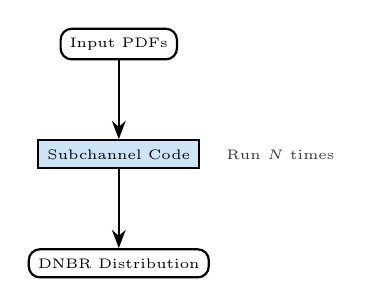
\begin{tikzpicture}[node distance=1.0cm, font=\tiny, thick]
            \node[draw, rectangle, rounded corners] (inputs) {Input PDFs};
            \node[draw, rectangle, fill=HadronBlue!20, below=of inputs] (code) {Subchannel Code};
            \node[draw, rectangle, rounded corners, below=of code] (output) {DNBR Distribution};
            \draw[-{Stealth}] (inputs) -- (code);
            \draw[-{Stealth}] (code) -- (output);
            \node[right=0.2cm of code, align=left, color=StatusDark] {Run $N$ times};
        \end{tikzpicture}
        }
        
        \vspace{0.3em}
        
        % Bottom: Margin Definition Image (ADDED)
        % Ensure filename is "margin_definition.png"
        \includegraphics[width=0.85\linewidth, keepaspectratio]{media/margin_definition.png}
        
        \vspace{0.2em}
        \tiny \textbf{Target: 95/95 Confidence/Probability}
    \end{columns}
\end{frame}

% ==========================================
% SLIDE 23: OPERATIONAL RESPONSE WORKFLOW
% ==========================================
\begin{frame}[t]{Operational Response Workflow}
    \centering
    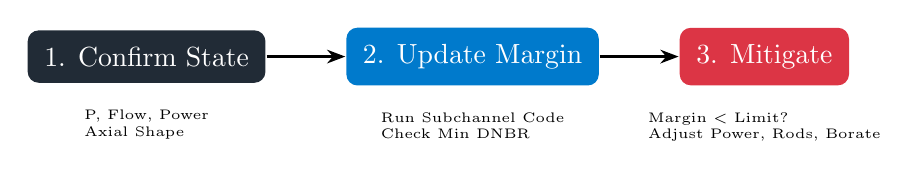
\begin{tikzpicture}[node distance=1.5cm, auto, thick]
        \node[fill=HadronDark, text=white, rounded corners, inner sep=6pt] (step1) {1. Confirm State};
        \node[fill=HadronBlue, text=white, rounded corners, inner sep=6pt, right=1cm of step1] (step2) {2. Update Margin};
        \node[fill=StatusRed, text=white, rounded corners, inner sep=6pt, right=1cm of step2] (step3) {3. Mitigate};

        \draw[-{Stealth}] (step1) -- (step2);
        \draw[-{Stealth}] (step2) -- (step3);
        
        \node[below=0.2cm of step1, align=left, font=\tiny] {P, Flow, Power\\Axial Shape};
        \node[below=0.2cm of step2, align=left, font=\tiny] {Run Subchannel Code\\Check Min DNBR};
        \node[below=0.2cm of step3, align=left, font=\tiny] {Margin < Limit?\\Adjust Power, Rods, Borate};
    \end{tikzpicture}

    \vspace{1.5cm}
    \statusbadge{StatusDark}{Principle: Proactive Margin Management}
\end{frame}

% ==========================================
% SLIDE 24: MITIGATION STRATEGIES
% ==========================================
\begin{frame}[t]{Mitigation Strategies}
    \begin{columns}[T,onlytextwidth]
        \column{0.50\textwidth}
        \textbf{Immediate Actions (Control Room)}
        \begin{itemize}
            \item \textbf{Reduce Power:} Direct heat flux reduction.
            \item \textbf{Increase Flow:} Improves rewetting and entrainment margin.
            \item \textbf{Shape Control:} Use rods to flatten axial peaks.
        \end{itemize}

        \column{0.45\textwidth}
        \textbf{Long-Term Engineering}
        \begin{itemize}
            \item \textbf{Spacer Design:} Enhance deposition (mixing vanes).
            \item \textbf{Fuel Cycle:} Load patterns to minimize peaking.
            \item \textbf{Chemistry:} Prevent crud buildup.
        \end{itemize}
    \end{columns}
\end{frame}

% ==========================================
% SLIDE 25: FINAL TAKEAWAYS
% ==========================================
\begin{frame}[t]{Final Takeaways}
    \begin{itemize}
        \item \textbf{Physics:} It's about liquid contact. DNB (bubbles blocking) vs Dryout (film exhaustion).
        \item \textbf{Modeling:} 3-Field models are essential for high-quality BWR analysis to track the film.
        \item \textbf{Safety:} Margins are statistical. We operate far from the cliff to account for uncertainty.
    \end{itemize}
    
    \vspace{2em}
    \centering
    \includegraphics[width=3cm]{media/hadron_logo.png} \\
    {\tiny \textbf{Hadron Energy Operations}}
\end{frame}

% ==========================================
% SLIDE 26: REFERENCES
% ==========================================
\begin{frame}[t]{References \& Further Reading}
    \begin{columns}[T,onlytextwidth]
        \column{0.65\textwidth}
        \textbf{Key Technical Resources}
        \begin{itemize}
            \item \textbf{Textbooks:}
            \begin{itemize} \small
                \item Todreas, N.E. \& Kazimi, M.S. \emph{Nuclear Systems Vol I}.
                \item Lahey, R.T. \& Moody, F.J. \emph{Thermal-Hydraulics of a BWR}.
            \end{itemize}
            \vspace{0.5em}
            \item \textbf{Methodology:}
            \begin{itemize} \small
                \item "COBRA-TF: A Three-Field Two-Fluid Model."
                \item EPRI Reports on CHF correlations.
            \end{itemize}
        \end{itemize}

        \column{0.32\textwidth}
        \textbf{Industry Codes}
        \vspace{0.5em}
        \statusbadge{HadronBlue}{VIPRE-01} \vspace{0.3em} \\
        \statusbadge{HadronBlue}{COBRA-TF (CTF)} \vspace{0.3em} \\
        \statusbadge{HadronBlue}{RELAP5-3D}
    \end{columns}
\end{frame}

\end{document}

